%----------------------------------------------------------------------------------------
%       ANEXO B: ARTÍCULOS PUBLICADOS
%----------------------------------------------------------------------------------------
\chapter{Artículos Publicados}
\label{anexo:articulos_publicados}

Este anexo presenta los artículos científicos publicados como resultado de la investigación realizada en esta tesis. Los trabajos fueron publicados en revistas arbitradas con registro ISSN y abordan el método de mejora de contraste mediante expansión estadística asimétrica de histograma (SAHS), una técnica de preprocesamiento complementaria a la normalización geométrica desarrollada en este trabajo.

\section{Artículo en Revista Internacional (Inglés)}

El siguiente artículo fue publicado en una revista científica internacional arbitrada. El trabajo describe el método SAHS (Statistical Asymmetrical Histogram Stretching) para mejora de contraste en imágenes de rayos X de tórax, el cual se combina con un algoritmo localizador de pulmones (ALP) para mejorar la detección de neumonía utilizando redes neuronales convolucionales.

\textbf{Título:} Statistical Asymmetrical Histogram Stretching for Contrast Enhancement in Chest X-ray Images for Pneumonia Detection

\textbf{Autores:} Rafael Alejandro Cruz Ovando\textsuperscript{1}, Salvador E. Ayala Raggi\textsuperscript{1}, Ángel E. Picazo Castillo\textsuperscript{2}, Aldrin Barreto Flores\textsuperscript{1}, José Francisco Portillo Robledo\textsuperscript{1}

\textbf{Afiliaciones:}
\begin{enumerate}
\item Benemérita Universidad Autónoma de Puebla, México
\item Instituto Nacional de Astrofísica, Óptica y Electrónica (INAOE), México
\end{enumerate}

\textbf{Revista:} Computación y Sistemas, Vol. 29, No. 4, 2025, pp. 2211–2222

\textbf{DOI:} 10.13053/CyS-29-4-6115

\textbf{ISSN:} 2007-9737

\textbf{Fechas:} Recibido: 01/06/2025, Aceptado: 02/10/2025

\textbf{Resumen:} Este artículo presenta un enfoque para mejorar el contraste en imágenes de rayos X de tórax mediante la técnica SAHS, que aborda la asimetría inherente en los histogramas de este tipo de imágenes. El método se evalúa en diversas arquitecturas CNN (AlexNet, Compact, Enhanced, ResNet-18, MobileNetV2, ResNet-50) y demuestra mejoras consistentes en la precisión de clasificación de neumonía, particularmente en la preservación de regiones brillantes diagnósticamente relevantes.

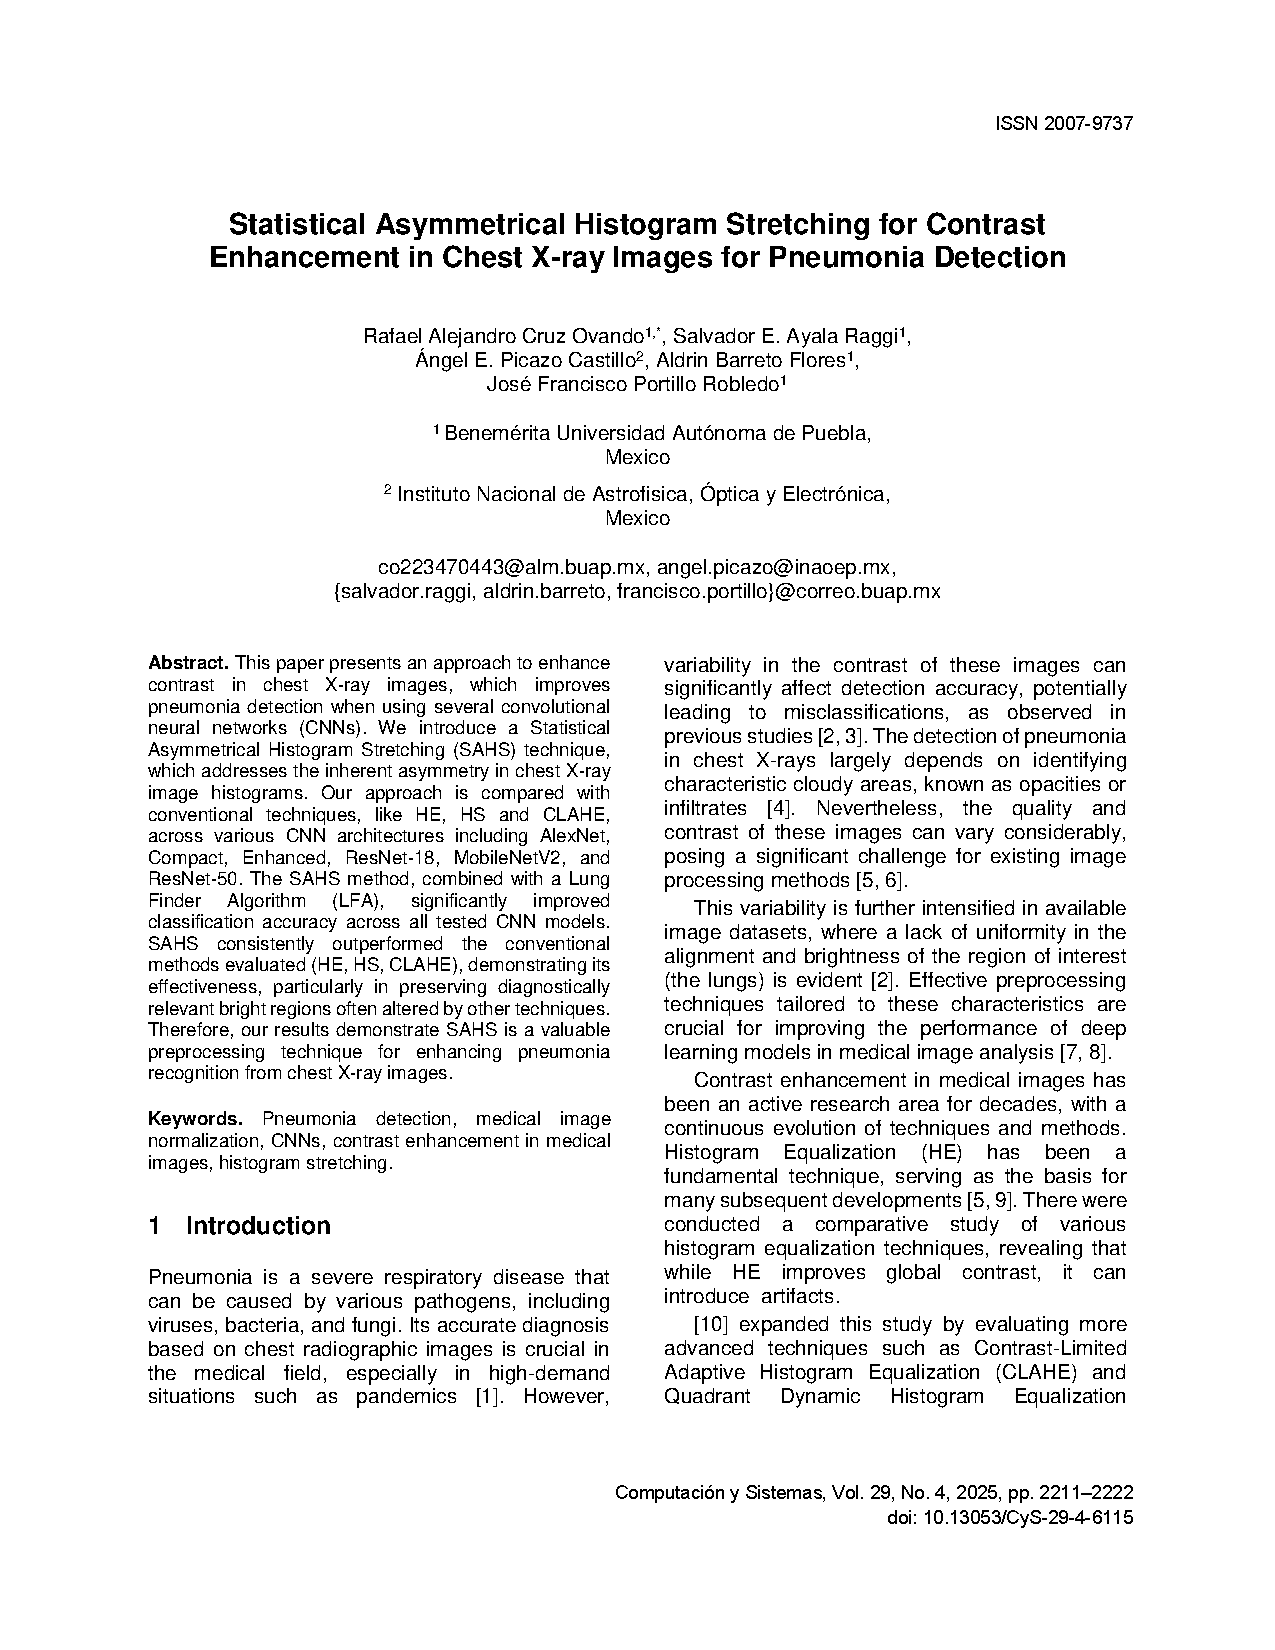
\includepdf[pages=-,pagecommand={\thispagestyle{plain}}]{anexos/articulo_ingles_sahs_2024.pdf}

\section{Artículo en Revista Nacional (Español)}

El siguiente artículo corresponde a la versión en español del trabajo anterior, publicado en una revista científica nacional.

\textbf{Título:} Enfoque de expansión estadística de histograma asimétrico para mejorar el contraste en imágenes de radiografías de tórax para la detección de neumonía

\textbf{Autores:} Rafael Alejandro Cruz Ovando\textsuperscript{1}, Salvador E. Ayala Raggi\textsuperscript{1}, Ángel E. Picazo Castillo\textsuperscript{2}, Aldrin Barreto Flores\textsuperscript{1}, José Francisco Portillo Robledo\textsuperscript{1}

\textbf{Afiliaciones:}
\begin{enumerate}
\item Benemérita Universidad Autónoma de Puebla, Av. San Claudio s/n, Cd Universitaria, C.P. 72592, Puebla, Puebla, México
\item Instituto Nacional de Astrofísica, Óptica y Electrónica, Luis Enrique Erro \#1, C.P. 72840, Sta. María Tonantzintla, Puebla, México
\end{enumerate}

\textbf{Revista:} Abstraction \& Application, Vol. 48, 2024, pp. 133–143

\textbf{Clasificación:} 2020 Mathematics Subject Classification: 68N01

\textbf{Palabras clave:} Detección de Neumonía, Normalización de Imágenes Médicas, CNNs, Mejora de Contraste en Imágenes Médicas, Expansión de Histograma

\textbf{Fechas:} Recibido: 5 de agosto, 2024; Aceptado: 7 de octubre, 2024

\textbf{Resumen:} Este trabajo presenta la técnica SAHS (Statistical Asymmetrical Histogram Stretching) para mejorar el contraste en imágenes de radiografías de tórax, abordando la asimetría inherente en los histogramas de este tipo de imágenes. El método se compara con técnicas convencionales (HE, CLAHE) en diversas arquitecturas CNN, demostrando su eficacia en preservar información crítica como regiones brillantes que indican neumonía. Los resultados muestran que SAHS supera consistentemente a CLAHE en la mayoría de los casos evaluados.

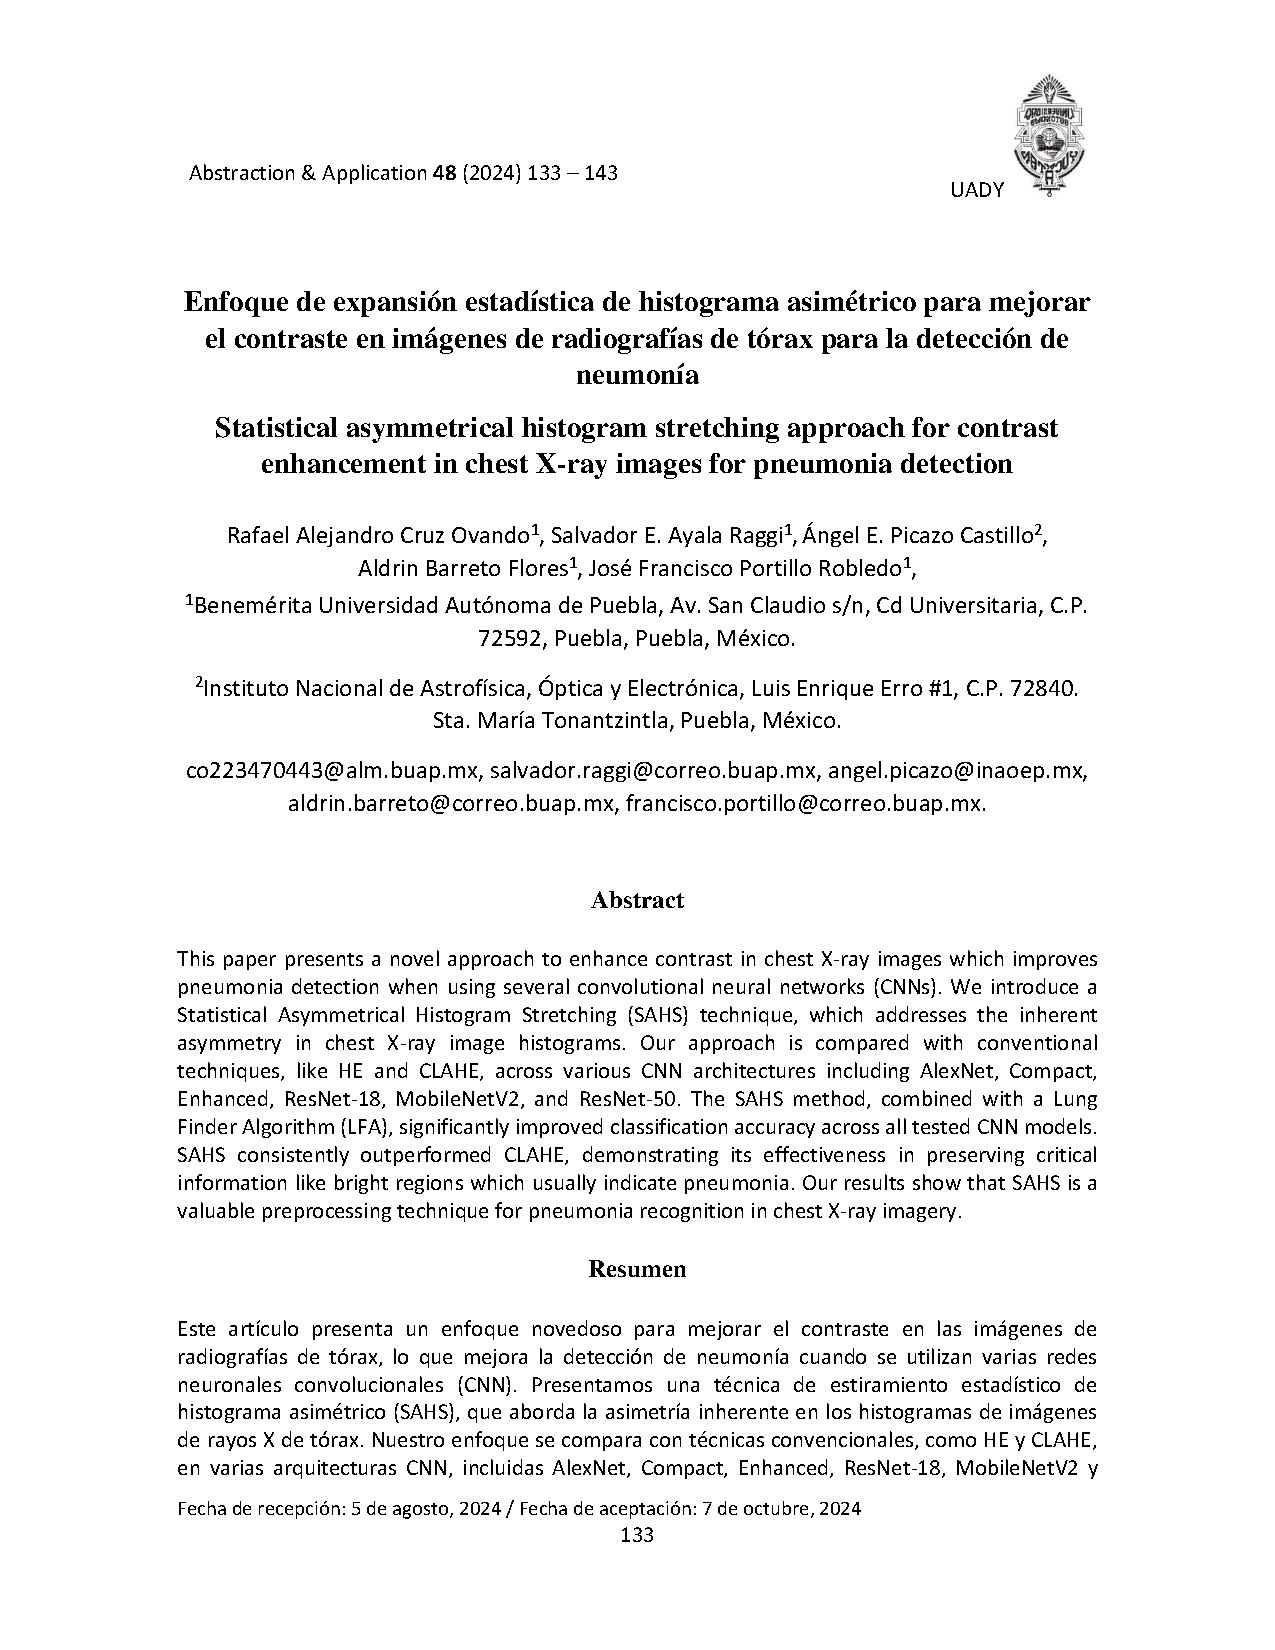
\includepdf[pages=-,pagecommand={\thispagestyle{plain}}]{anexos/articulo_espanol_sahs_2024.pdf}
